\chapter{Analyse}

\section{Softwarearchitektur des Radarsimulators}
Im folgenden Abschnitt werden die einzelnen Softwarekomponenten der Radarsimulator Anwendung beschrieben und auf Wiederverwendbarkeit und Modularität überprüft. Dabei wird sich auf die Kernkomponenten der Anwendung beschränkt.

Der Radar Simulator ist eine Eclipse RCP Anwendung. Das Modul, das die Benutzeroberfläche zur Verfügung stellt, ist der RadarSimulator.app. Darin werden die Startinformationen und weitere Fenstereinstellungen für diese Anwendungen angegeben. Der Startpunkt der Anwendung ist die SimulatorMain Klasse. Diese startet das Backend und Frontend. Zudem besitzt der Radarsimulator einen Restart Service. Dieser Service ermöglicht es, die Simulation über ein Fenster Menü item neu zu starten. Dabei wird die Benutzeroberfläche und die Simulator Instanz neu geladen. Diese Funktion ist in der SimulatorMain Klasse implementiert.

\begin{figure}[h]
    \centering
    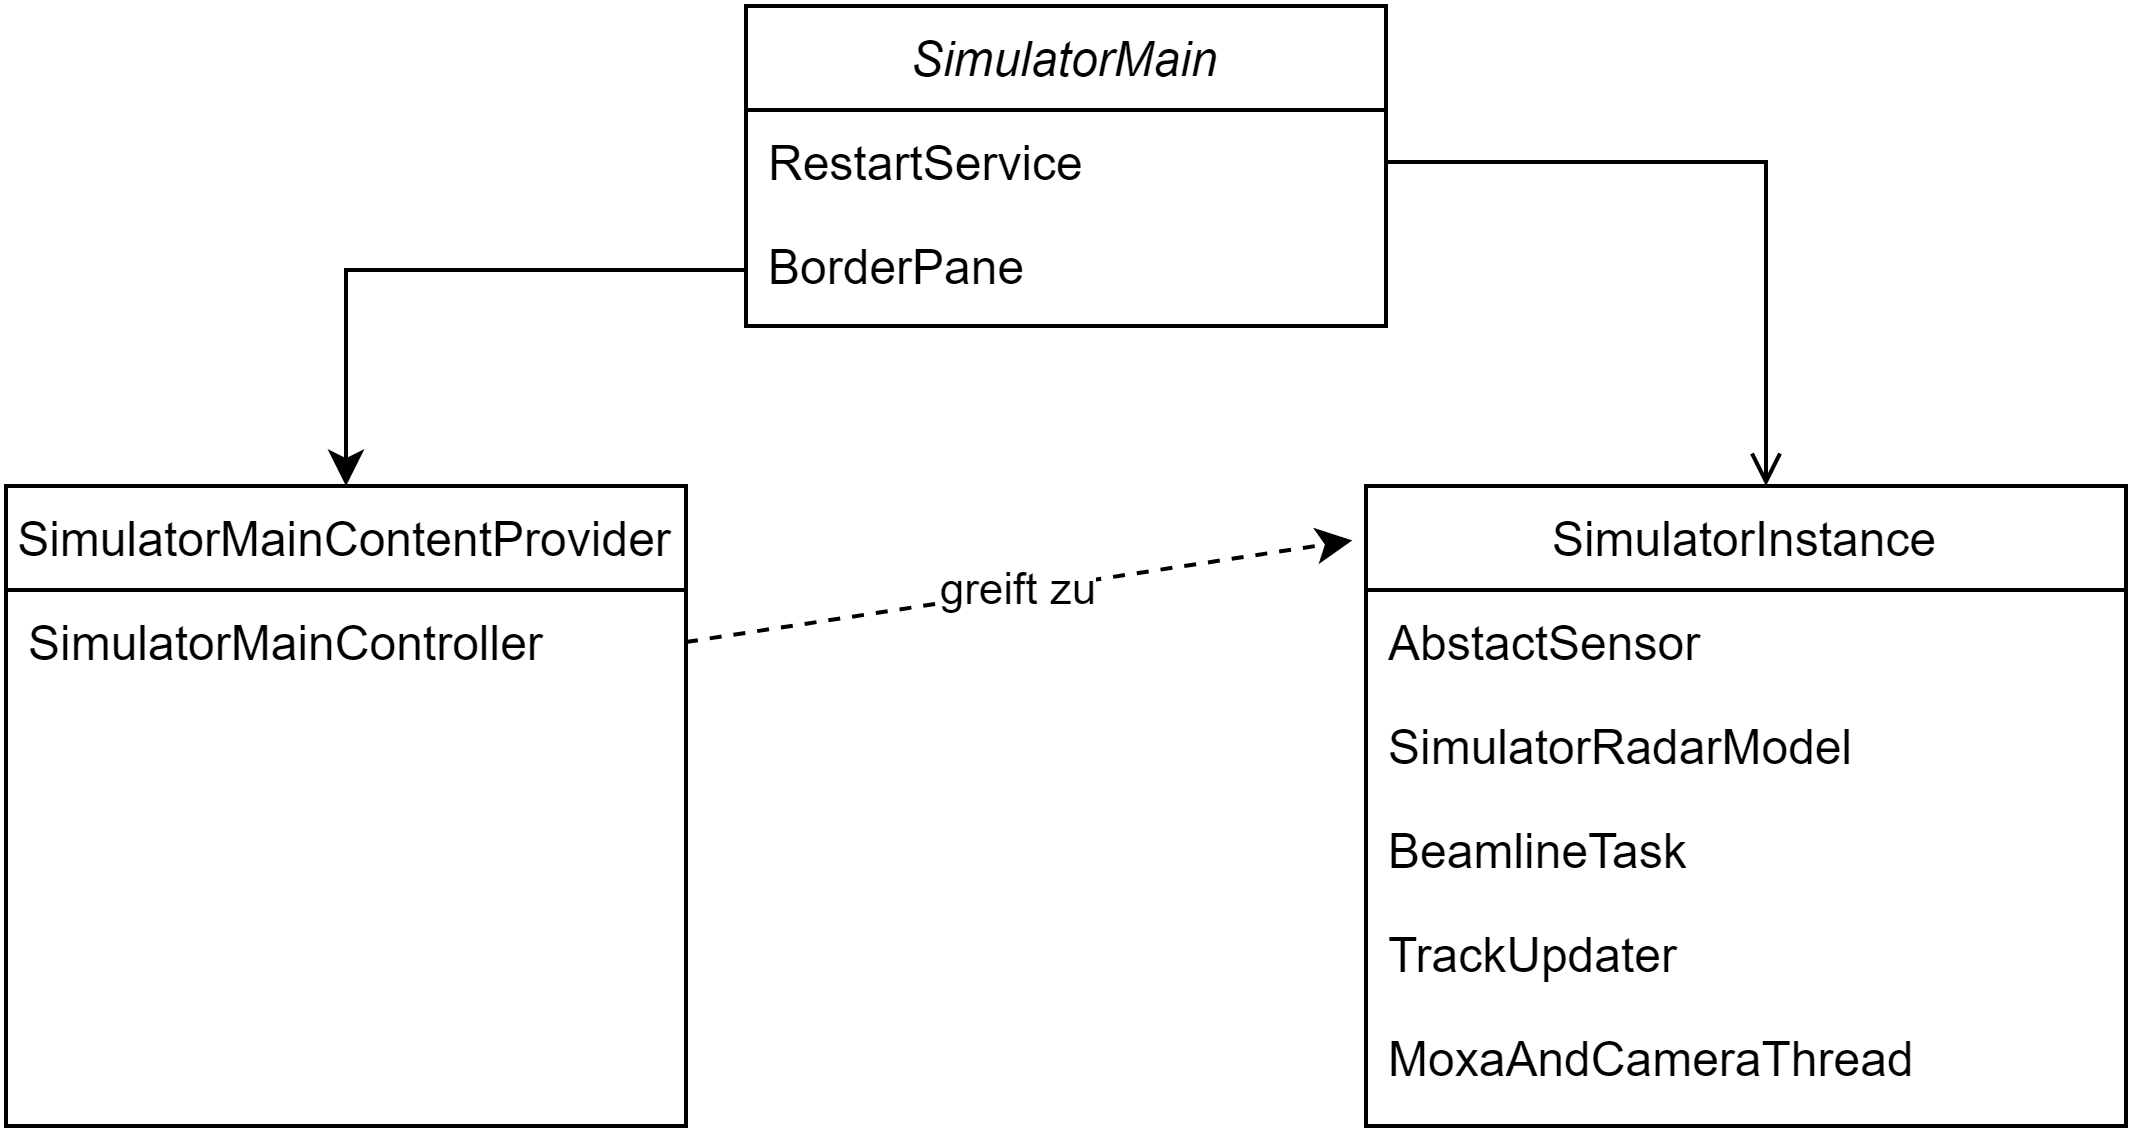
\includegraphics[width=0.8\textwidth]{content/assets/RadarSimulatorUML.png}
    \caption{UML-Diagramm des Radarsimulators}
\end{figure}